\documentclass[a4paper,11pt]{article}

\usepackage[utf8]{inputenc}

\usepackage{minted}

\usepackage{graphicx}
\usepackage{caption}
\usepackage{subcaption}
\usepackage{placeins}
\usepackage{pgfplots}
\pgfplotsset{compat=1.18} 

\begin{document}

\title{
    \textbf{Environment}
}
\author{Jonathan Karlsson}
\date{Spring Term 2023}

\maketitle

\section*{Introduction}
The task for this assignment was to create two different versions of a key value data structure, one in the form of a list and one in the form of a tree.

\section*{Implementation}
\subsection*{List}
The implementation required four functions, new, add, lookup and remove. The first way the key values were stored was using a list, where each key value would be added to the list as an element. New was the first function to be implemented, it would simply return a empty list. 
The second function was add. This was implemented by first checking if the inputted list was empty, if it was the key,value pair was simply added to it. If it was not empty another add function was called with the same arguments as the first plus a second list. This second add would run through the first list and copy it to the second until either the key was found and the key value was inserted instead of the original key value or the list ended, where it would then be added to the end. 
The new list would then be returned.
\begin{minted}{elixir}
def add([h|t],key,value,new_map) do

  case t do
    [] -> case h do
      {^key,_} -> new_map = new_map++[{key,value}]; new_map
      _ -> new_map = new_map++[h,{key,value}];new_map
    end

    _ -> case h do
      {^key,_} -> new_map = new_map++[{key,value}|t]; new_map
      _ ->  new_map = new_map++[h]; add(t,key,value,new_map)
    end
  end
end
    
\end{minted}
The second function, the lookup was just made as a single function where it would check if the head of the list was the key it was looking for, otherwise it would either call itself with the tail or return nil if there was no more tail.
\begin{minted}{elixir}
def lookup([h|t],key) do
  case h do
    {^key,_} -> h
    _ -> case t do
      [] -> :nil
      _ -> lookup(t,key)
    end
  end
end
    
\end{minted}
The final function for the list implementation was the remove. This was implemented in a similar way to the add where it would call a second remove with a new empty list, then copy everything to that list except the elements that contain the key. Then the new list is returned when there is nothing more to copy.
\begin{minted}{elixir}
def remove(key,[h|t],new_map) do
  case t do
    [] -> case h do
        {^key,_} -> new_map
        _ -> new_map = new_map++[h];new_map
    end
    _ -> case h do
        {^key,_} -> remove(key,t,new_map)
        _ ->  new_map = new_map++[h]; remove(key,t,new_map)
    end
  end
end
\end{minted}
\subsection*{Tree}
The was a bit more complicated to implement than the as each function needed different cases to determine where the key value pair was and what to do with it. The simplest function to implement was once again the new as that function only had to return a nil. The second function was the add, this function required some conditions, so multiple definitions of the function was written. The first of the add functions was the case where the current node is nil, then add should just add a node att this spot which it does by returning a new node with no right or left branch. 
The second add checks if the key in the current node is the same as the key that wants to be put into the tree, if it is the node is replaced by returning a new node with the same left and right as the previous node. The last two are very similar, the first one checks if the key is lower than the current key, if it is the returned node has another add in its left branch as the added node has to be to the left. The final one has the new add on the right and no conditional as it is already known that it should not be on the left as the previous condition was false.
\begin{minted}{elixir}
def add(nil, key, value) do
    {:node,key,value,:nil,:nil}
end
def add({:node, key, _, left, right}, key, value) do
    {:node,key,value,left,right}
end
def add({:node, k, v, left, right}, key, value) when key < k do
    {:node,k,v,add(left,key,value),right}
end
def add({:node, k, v, left, right}, key, value) do
    {:node,k,v,left,add(right,key,value)}
end
\end{minted}
The lookup also requires different cases The first one being that the current node is nil, then the lookup returns nil, if the current node has the key that is searched for the key and value is returned. finally the last two lookup functions calls lookup on either the left or right branch depending on if the key is smaller or larger than the one looked for the result from either the first or second lookup function then gets recursively returned.
\begin{minted}{elixir}
def lookup({:node, key, v, _, _}, key) do
    {key,v}
end
def lookup({:node, k, _, left, _}, key) when key < k do
    lookup(left,key)
end
def lookup({:node, _, _, _, right}, key) do
    lookup(right,key)
end
\end{minted}
The remove function was the most complicated to implement as it required moving the leftmost node from the right branch into the current position. The first three functions were simple however, the first one was when the node is nil then nil is returned. The second is when the node that is wanted does not have a node to its left then the node is replaced with the node to the right. The same is true for the third function when the node does not have a node to the right the node is replaced with the node to the left.
The fourth function returns the node with the key value and right of the node that was the leftmost from the right branch, as this will replace the current node with that node, however the left branch still need to be kept as anything larger than the removed node, which is the right branch will also be larger than whatever is one the left of the replaced node. Getting the leftmost means getting the smallest node to the right of the current node. 
The fifth and sixth functions navigate to the node to be removed in the same way add navigated to the node to be added or changed.
\begin{minted}{elixir}
def remove({:node, key, _, left, right}, key) do
    {:node, new_key,new_value,_,new_right} = leftmost(right)
    {:node, new_key, new_value, left ,new_right}
end
def remove({:node, k, v, left, right}, key) when key < k do
    {:node, k, v, remove(left,key), right}
end
def remove({:node, k, v, left, right}, key) do
    {:node, k, v, left, remove(right,key)}
end
\end{minted}
The leftmost function consists of two functions. The first one is when the left most is found as the left path is nil, then the node is returned. The second one recursively calls leftmost with the left node then returns the key, value and left from the found node. It also sets the right path of the returned node as the current node with its left replaced with the right of the found node. 
\begin{minted}{elixir}
def leftmost({:node, key, value, nil, rest}) do
    {:node,key,value,:nil,rest}
end
def leftmost({:node, k, v, left, right}) do
    {:node, new_key,new_value,new_left,new_right} = leftmost(left)
    {:node,new_key,new_value,new_left,{:node, k, v, new_right, right}}
end
\end{minted}

\section*{Benchmark}
The benchmark was split into three parts, the list, the tree and the inbuilt Map function. The first benchmark for the list was done with 100 operations.

\begin{table}[h]
    \begin{center}
    \scalebox{1}{
    \begin{tabular}{l|c|c|c}
    \textbf{n} & \textbf{add({\textmu}s)} & \textbf{lookup({\textmu}s)}& \textbf{remove({\textmu}s)}\\
    \hline
    16 &       0.00&        1.02&        0.00 \\
    32 &       1.02&        0.00&        0.00 \\
    64 &       1.02&        0.00&        1.02 \\
   128 &       4.09&        0.00&        6.14 \\
   256 &      10.24&        0.00&       19.45 \\
   512 &      52.22&        1.02&       82.94 \\
  1024 &     239.61&        0.00&      397.31 \\
  2048 &     841.72&        1.02&     1492.99 \\
  4096 &    4453.37&        3.07&     5852.16 \\
  8192 &   33419.26&        6.14&    55868.41 \\   
    \end{tabular}
    }
    \caption{The result of the list benchmark when run using 100 operations}
    \label{tab:table1}
    \end{center}
\end{table}

\FloatBarrier{\noindent}
A graph to visualize the result was also created for each of the benchmarks here is the graph for the list.

\begin{figure}[h]
    \centering    
    
    \scalebox{0.8}{% GNUPLOT: LaTeX picture with Postscript
\begingroup
  \makeatletter
  \providecommand\color[2][]{%
    \GenericError{(gnuplot) \space\space\space\@spaces}{%
      Package color not loaded in conjunction with
      terminal option `colourtext'%
    }{See the gnuplot documentation for explanation.%
    }{Either use 'blacktext' in gnuplot or load the package
      color.sty in LaTeX.}%
    \renewcommand\color[2][]{}%
  }%
  \providecommand\includegraphics[2][]{%
    \GenericError{(gnuplot) \space\space\space\@spaces}{%
      Package graphicx or graphics not loaded%
    }{See the gnuplot documentation for explanation.%
    }{The gnuplot epslatex terminal needs graphicx.sty or graphics.sty.}%
    \renewcommand\includegraphics[2][]{}%
  }%
  \providecommand\rotatebox[2]{#2}%
  \@ifundefined{ifGPcolor}{%
    \newif\ifGPcolor
    \GPcolortrue
  }{}%
  \@ifundefined{ifGPblacktext}{%
    \newif\ifGPblacktext
    \GPblacktextfalse
  }{}%
  % define a \g@addto@macro without @ in the name:
  \let\gplgaddtomacro\g@addto@macro
  % define empty templates for all commands taking text:
  \gdef\gplbacktext{}%
  \gdef\gplfronttext{}%
  \makeatother
  \ifGPblacktext
    % no textcolor at all
    \def\colorrgb#1{}%
    \def\colorgray#1{}%
  \else
    % gray or color?
    \ifGPcolor
      \def\colorrgb#1{\color[rgb]{#1}}%
      \def\colorgray#1{\color[gray]{#1}}%
      \expandafter\def\csname LTw\endcsname{\color{white}}%
      \expandafter\def\csname LTb\endcsname{\color{black}}%
      \expandafter\def\csname LTa\endcsname{\color{black}}%
      \expandafter\def\csname LT0\endcsname{\color[rgb]{1,0,0}}%
      \expandafter\def\csname LT1\endcsname{\color[rgb]{0,1,0}}%
      \expandafter\def\csname LT2\endcsname{\color[rgb]{0,0,1}}%
      \expandafter\def\csname LT3\endcsname{\color[rgb]{1,0,1}}%
      \expandafter\def\csname LT4\endcsname{\color[rgb]{0,1,1}}%
      \expandafter\def\csname LT5\endcsname{\color[rgb]{1,1,0}}%
      \expandafter\def\csname LT6\endcsname{\color[rgb]{0,0,0}}%
      \expandafter\def\csname LT7\endcsname{\color[rgb]{1,0.3,0}}%
      \expandafter\def\csname LT8\endcsname{\color[rgb]{0.5,0.5,0.5}}%
    \else
      % gray
      \def\colorrgb#1{\color{black}}%
      \def\colorgray#1{\color[gray]{#1}}%
      \expandafter\def\csname LTw\endcsname{\color{white}}%
      \expandafter\def\csname LTb\endcsname{\color{black}}%
      \expandafter\def\csname LTa\endcsname{\color{black}}%
      \expandafter\def\csname LT0\endcsname{\color{black}}%
      \expandafter\def\csname LT1\endcsname{\color{black}}%
      \expandafter\def\csname LT2\endcsname{\color{black}}%
      \expandafter\def\csname LT3\endcsname{\color{black}}%
      \expandafter\def\csname LT4\endcsname{\color{black}}%
      \expandafter\def\csname LT5\endcsname{\color{black}}%
      \expandafter\def\csname LT6\endcsname{\color{black}}%
      \expandafter\def\csname LT7\endcsname{\color{black}}%
      \expandafter\def\csname LT8\endcsname{\color{black}}%
    \fi
  \fi
    \setlength{\unitlength}{0.0500bp}%
    \ifx\gptboxheight\undefined%
      \newlength{\gptboxheight}%
      \newlength{\gptboxwidth}%
      \newsavebox{\gptboxtext}%
    \fi%
    \setlength{\fboxrule}{0.5pt}%
    \setlength{\fboxsep}{1pt}%
    \definecolor{tbcol}{rgb}{1,1,1}%
\begin{picture}(7200.00,5040.00)%
    \gplgaddtomacro\gplbacktext{%
      \csname LTb\endcsname%%
      \put(1078,771){\makebox(0,0)[r]{\strut{}$0$}}%
      \put(1078,1446){\makebox(0,0)[r]{\strut{}$10000$}}%
      \put(1078,2121){\makebox(0,0)[r]{\strut{}$20000$}}%
      \put(1078,2795){\makebox(0,0)[r]{\strut{}$30000$}}%
      \put(1078,3470){\makebox(0,0)[r]{\strut{}$40000$}}%
      \put(1078,4144){\makebox(0,0)[r]{\strut{}$50000$}}%
      \put(1078,4819){\makebox(0,0)[r]{\strut{}$60000$}}%
      \put(1210,484){\makebox(0,0){\strut{}$0$}}%
      \put(1831,484){\makebox(0,0){\strut{}$1000$}}%
      \put(2453,484){\makebox(0,0){\strut{}$2000$}}%
      \put(3074,484){\makebox(0,0){\strut{}$3000$}}%
      \put(3696,484){\makebox(0,0){\strut{}$4000$}}%
      \put(4317,484){\makebox(0,0){\strut{}$5000$}}%
      \put(4939,484){\makebox(0,0){\strut{}$6000$}}%
      \put(5560,484){\makebox(0,0){\strut{}$7000$}}%
      \put(6182,484){\makebox(0,0){\strut{}$8000$}}%
      \put(6803,484){\makebox(0,0){\strut{}$9000$}}%
    }%
    \gplgaddtomacro\gplfronttext{%
      \csname LTb\endcsname%%
      \put(209,2761){\rotatebox{-270}{\makebox(0,0){\strut{}time in µs}}}%
      \put(4006,154){\makebox(0,0){\strut{}n}}%
      \csname LTb\endcsname%%
      \put(2134,4646){\makebox(0,0)[r]{\strut{}add}}%
      \csname LTb\endcsname%%
      \put(2134,4426){\makebox(0,0)[r]{\strut{}lookup}}%
      \csname LTb\endcsname%%
      \put(2134,4206){\makebox(0,0)[r]{\strut{}remove}}%
    }%
    \gplbacktext
    \put(0,0){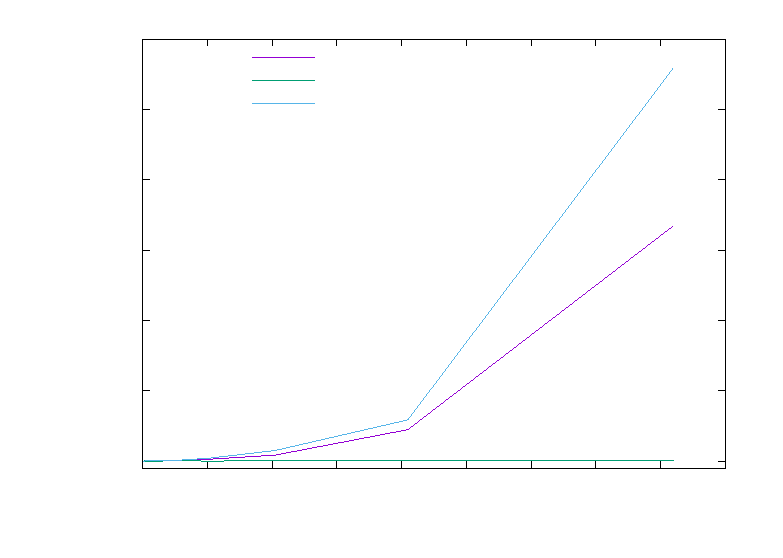
\includegraphics[width={360.00bp},height={252.00bp}]{listb}}%
    \gplfronttext
  \end{picture}%
\endgroup
}
    \caption{Visualization of the list running 100 operations}   
    \label{tab:figure1} 
    
    \end{figure}
\FloatBarrier{\noindent}

It is obvious that the lookup is much faster than the add or the remove, this is probably because the lookup only has to go through the list once while the add and remove has to copy the list multiple times, this is obviously not efficient.

Due to the tree version being much faster the tree has 10000 operations instead of 100 to produce meaningful results. 
\begin{table}[h]
    \begin{center}
    \scalebox{1}{
    \begin{tabular}{l|c|c|c}
    \textbf{n} & \textbf{add({\textmu}s)} & \textbf{lookup({\textmu}s)}& \textbf{remove({\textmu}s)}\\
    \hline
    16     &   0.05&        0.02 &       0.02 \\
    32     &   0.04&        0.03 &       0.03 \\
    64     &   0.05&        0.03 &       0.05 \\
   128     &   0.08&        0.04 &       0.06 \\
   256     &   0.06&        0.05 &       0.09 \\
   512     &   0.07&        0.05 &       0.08 \\
  1024     &   0.09&        0.06 &       0.11 \\
  2048     &   0.09&        0.06 &       0.11 \\
  4096     &   0.10&        0.09 &       0.13 \\
  8192     &   0.12&        0.08 &       0.14 \\
    \end{tabular}
    }
    \caption{The result of the tree benchmark when run using 10000 operations}
    \label{tab:table2}
    \end{center}
\end{table}
\FloatBarrier{\noindent}
Finally the inbuilt Map function was benchmarked using the same benchmark as the tree and the list and also using 10000 operations.
\begin{table}[h]
    \begin{center}
    \scalebox{1}{
    \begin{tabular}{l|c|c|c}
    \textbf{n} & \textbf{add({\textmu}s)} & \textbf{lookup({\textmu}s)}& \textbf{remove({\textmu}s)}\\
    \hline
    16     &   0.02 &       0.02 &       0.01 \\
    32     &   0.04 &       0.02 &       0.01 \\
    64     &   0.03 &       0.02 &       0.03 \\
   128     &   0.04 &       0.02 &       0.02 \\
   256     &   0.06 &       0.02 &       0.03 \\
   512     &   0.05 &       0.02 &       0.03 \\
  1024     &   0.05 &       0.02 &       0.04 \\
  2048     &   0.04 &       0.02 &       0.04 \\
  4096     &   0.09 &       0.02 &       0.04 \\
  8192     &   0.07 &       0.02 &       0.07 \\
    \end{tabular}
    }
    \caption{The result of the Map benchmark when run using 10000 operations}
    \label{tab:table3}
    \end{center}
\end{table}
\FloatBarrier{\noindent}
The inbuilt function is slightly faster than the tree function created, it also seems to have a constant time for lookup while the tree function has an increasing time for the lookup. 
Both tree and Map was inserted into a graph visualized below for Visualization of the differences between them.
\begin{figure}[h]
    \centering    
    
    \scalebox{0.8}{% GNUPLOT: LaTeX picture with Postscript
\begingroup
  \makeatletter
  \providecommand\color[2][]{%
    \GenericError{(gnuplot) \space\space\space\@spaces}{%
      Package color not loaded in conjunction with
      terminal option `colourtext'%
    }{See the gnuplot documentation for explanation.%
    }{Either use 'blacktext' in gnuplot or load the package
      color.sty in LaTeX.}%
    \renewcommand\color[2][]{}%
  }%
  \providecommand\includegraphics[2][]{%
    \GenericError{(gnuplot) \space\space\space\@spaces}{%
      Package graphicx or graphics not loaded%
    }{See the gnuplot documentation for explanation.%
    }{The gnuplot epslatex terminal needs graphicx.sty or graphics.sty.}%
    \renewcommand\includegraphics[2][]{}%
  }%
  \providecommand\rotatebox[2]{#2}%
  \@ifundefined{ifGPcolor}{%
    \newif\ifGPcolor
    \GPcolortrue
  }{}%
  \@ifundefined{ifGPblacktext}{%
    \newif\ifGPblacktext
    \GPblacktextfalse
  }{}%
  % define a \g@addto@macro without @ in the name:
  \let\gplgaddtomacro\g@addto@macro
  % define empty templates for all commands taking text:
  \gdef\gplbacktext{}%
  \gdef\gplfronttext{}%
  \makeatother
  \ifGPblacktext
    % no textcolor at all
    \def\colorrgb#1{}%
    \def\colorgray#1{}%
  \else
    % gray or color?
    \ifGPcolor
      \def\colorrgb#1{\color[rgb]{#1}}%
      \def\colorgray#1{\color[gray]{#1}}%
      \expandafter\def\csname LTw\endcsname{\color{white}}%
      \expandafter\def\csname LTb\endcsname{\color{black}}%
      \expandafter\def\csname LTa\endcsname{\color{black}}%
      \expandafter\def\csname LT0\endcsname{\color[rgb]{1,0,0}}%
      \expandafter\def\csname LT1\endcsname{\color[rgb]{0,1,0}}%
      \expandafter\def\csname LT2\endcsname{\color[rgb]{0,0,1}}%
      \expandafter\def\csname LT3\endcsname{\color[rgb]{1,0,1}}%
      \expandafter\def\csname LT4\endcsname{\color[rgb]{0,1,1}}%
      \expandafter\def\csname LT5\endcsname{\color[rgb]{1,1,0}}%
      \expandafter\def\csname LT6\endcsname{\color[rgb]{0,0,0}}%
      \expandafter\def\csname LT7\endcsname{\color[rgb]{1,0.3,0}}%
      \expandafter\def\csname LT8\endcsname{\color[rgb]{0.5,0.5,0.5}}%
    \else
      % gray
      \def\colorrgb#1{\color{black}}%
      \def\colorgray#1{\color[gray]{#1}}%
      \expandafter\def\csname LTw\endcsname{\color{white}}%
      \expandafter\def\csname LTb\endcsname{\color{black}}%
      \expandafter\def\csname LTa\endcsname{\color{black}}%
      \expandafter\def\csname LT0\endcsname{\color{black}}%
      \expandafter\def\csname LT1\endcsname{\color{black}}%
      \expandafter\def\csname LT2\endcsname{\color{black}}%
      \expandafter\def\csname LT3\endcsname{\color{black}}%
      \expandafter\def\csname LT4\endcsname{\color{black}}%
      \expandafter\def\csname LT5\endcsname{\color{black}}%
      \expandafter\def\csname LT6\endcsname{\color{black}}%
      \expandafter\def\csname LT7\endcsname{\color{black}}%
      \expandafter\def\csname LT8\endcsname{\color{black}}%
    \fi
  \fi
    \setlength{\unitlength}{0.0500bp}%
    \ifx\gptboxheight\undefined%
      \newlength{\gptboxheight}%
      \newlength{\gptboxwidth}%
      \newsavebox{\gptboxtext}%
    \fi%
    \setlength{\fboxrule}{0.5pt}%
    \setlength{\fboxsep}{1pt}%
    \definecolor{tbcol}{rgb}{1,1,1}%
\begin{picture}(7200.00,5040.00)%
    \gplgaddtomacro\gplbacktext{%
      \csname LTb\endcsname%%
      \put(946,704){\makebox(0,0)[r]{\strut{}$0$}}%
      \put(946,1292){\makebox(0,0)[r]{\strut{}$0.02$}}%
      \put(946,1880){\makebox(0,0)[r]{\strut{}$0.04$}}%
      \put(946,2468){\makebox(0,0)[r]{\strut{}$0.06$}}%
      \put(946,3055){\makebox(0,0)[r]{\strut{}$0.08$}}%
      \put(946,3643){\makebox(0,0)[r]{\strut{}$0.1$}}%
      \put(946,4231){\makebox(0,0)[r]{\strut{}$0.12$}}%
      \put(946,4819){\makebox(0,0)[r]{\strut{}$0.14$}}%
      \put(1078,484){\makebox(0,0){\strut{}$0$}}%
      \put(1714,484){\makebox(0,0){\strut{}$1000$}}%
      \put(2350,484){\makebox(0,0){\strut{}$2000$}}%
      \put(2986,484){\makebox(0,0){\strut{}$3000$}}%
      \put(3622,484){\makebox(0,0){\strut{}$4000$}}%
      \put(4259,484){\makebox(0,0){\strut{}$5000$}}%
      \put(4895,484){\makebox(0,0){\strut{}$6000$}}%
      \put(5531,484){\makebox(0,0){\strut{}$7000$}}%
      \put(6167,484){\makebox(0,0){\strut{}$8000$}}%
      \put(6803,484){\makebox(0,0){\strut{}$9000$}}%
    }%
    \gplgaddtomacro\gplfronttext{%
      \csname LTb\endcsname%%
      \put(209,2761){\rotatebox{-270}{\makebox(0,0){\strut{}time in µs}}}%
      \put(3940,154){\makebox(0,0){\strut{}n}}%
      \csname LTb\endcsname%%
      \put(2662,4646){\makebox(0,0)[r]{\strut{}add}}%
      \csname LTb\endcsname%%
      \put(2662,4426){\makebox(0,0)[r]{\strut{}lookup}}%
      \csname LTb\endcsname%%
      \put(2662,4206){\makebox(0,0)[r]{\strut{}remove}}%
      \csname LTb\endcsname%%
      \put(2662,3986){\makebox(0,0)[r]{\strut{}add(Map)}}%
      \csname LTb\endcsname%%
      \put(2662,3766){\makebox(0,0)[r]{\strut{}lookup(Map)}}%
      \csname LTb\endcsname%%
      \put(2662,3546){\makebox(0,0)[r]{\strut{}remove(Map)}}%
    }%
    \gplbacktext
    \put(0,0){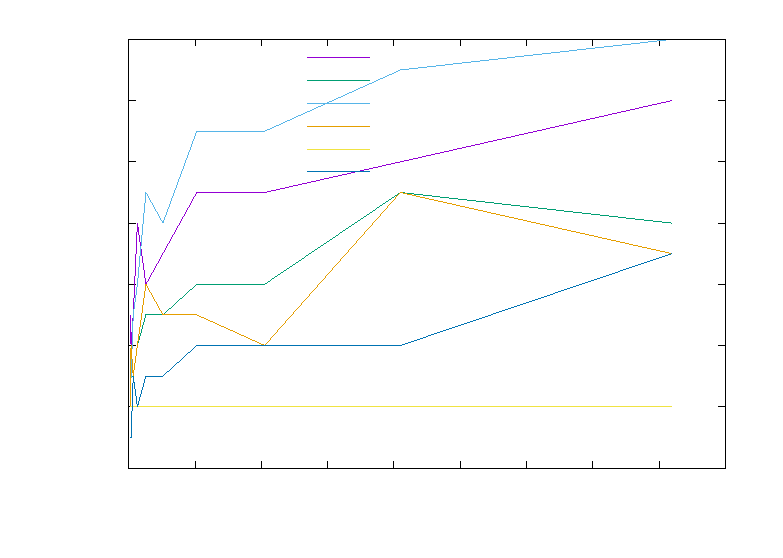
\includegraphics[width={360.00bp},height={252.00bp}]{treemapb}}%
    \gplfronttext
  \end{picture}%
\endgroup
}
    \caption{Visualization of the Map and tree running 10000 operations}   
    \label{tab:figure2} 
    
    \end{figure}
\FloatBarrier{\noindent}
\section*{Discussion}
It is obvious that the tree implementation is a lot faster than the list implementation. Even if the tree is a bit more complicated than the list to implement and understand it is definitely worth it to go for the tree as it was 
almost 280000 times faster while doing 100 times more add operations.


\end{document}
